\documentclass[25pt, a0paper, portrait, margin=0mm, innermargin=15mm,
     blockverticalspace=15mm, colspace=15mm, subcolspace=8mm]{tikzposter} 

\graphicspath{{figs/}}

% Font Setting
% --------------

\usepackage[hangul]{kotex}
\usepackage{fontspec}
\defaultfontfeatures{Numbers=OldStyle,Mapping=tex-text}

%Latin
\setmainfont{Minion Pro}
\setsansfont{Myriad Pro}

%Hnagul
\setmainhangulfont{나눔명조}
\setsanshangulfont{나눔고딕}

%Math
\usepackage[math]{iwona}


%Color
% Definerer 'NTNU-fargen', m?kebl?t, for bruk i bl.a. overskrifter.
\definecolor{NTNUBlue}{rgb}{0.0470,0,0.5294}
\definecolor{Apricot}     {cmyk}{0,0.32,0.52,0}
\definecolor{Aquamarine}  {cmyk}{0.82,0,0.30,0}
\definecolor{BrickRed}{cmyk}{0,0.89,0.94,0.28}
\definecolor{CadetBlue}   {cmyk}{0.62,0.57,0.23,0}
\definecolor{DarkGray}    {gray}{0.2}
\definecolor{DarkGreen}   {rgb}{0,0.5,0}
\definecolor{ForestGreen} {cmyk}{0.91,0,0.88,0.12}
\definecolor{Gold}        {rgb}{1.,0.84,0.}
\definecolor{Goldenrod}   {cmyk}{0,0.10,0.84,0}
\definecolor{IndianRed}   {rgb}{0.8,0.36,0.36}
\definecolor{Lavender}    {cmyk}{0,0.48,0,0}
\definecolor{LemonChiffon}{rgb}{1.,0.98,0.8}
\definecolor{LightBlue}   {rgb}{0.68,0.85,0.9}
\definecolor{LightCyan}   {rgb}{0.88,1.,1.}
\definecolor{LightGray}   {gray}{0.92}
\definecolor{LightYellow} {rgb}{1.,1.,0.88}
\definecolor{Melon}       {cmyk}{0,0.46,0.50,0}
\definecolor{NTNUBlue}{cmyk}{0.98,0.13,0,0.43}
\definecolor{NavyBlue}    {cmyk}{0.94,0.54,0,0}
\definecolor{Orange}      {rgb}{1.,0.65,0.}
\definecolor{PaleGreen}   {rgb}{0.6,0.98,0.6}
\definecolor{PaleGreenB}  {rgb}{0.9,1,0.9}
\definecolor{Peach}       {cmyk}{0,0.50,0.70,0}
\definecolor{PeachPuff}   {rgb}{1.0,0.85,0.73}
\definecolor{PineGreen}   {cmyk}{0.92,0,0.59,0.25}
\definecolor{Pink}        {rgb}{1.,0.75,0.8}
\definecolor{RoyalBlue}   {cmyk}{1,0.50,0,0}
\definecolor{SeaGreen}    {cmyk}{0.69,0,0.50,0}
\definecolor{Salmon}      {cmyk}{0,0.53,0.38,0}
\definecolor{Sepia}       {cmyk}{0,0.83,1,0.70}
\definecolor{SlateBlue}   {rgb}{0.42,0.35,0.8}
\definecolor{Thistle}     {rgb}{0.85,0.75,0.85}
\definecolor{Turquoise}   {cmyk}{0.85,0,0.20,0}
\definecolor{Violet}      {cmyk}{0.79,0.88,0,0}
\definecolor{YellowOrange}{cmyk}{0,0.42,1,0}

%Section Style
\def\mysection#1{\textbf{\Large\color{NTNUBlue}\sf #1}\par}

%Emph
\def\myem#1{\textsf{\color{BrickRed}#1}}


% LATEX PACKAGES
% --------------

\usepackage{amsmath}
\usepackage{graphicx}  % package for inserting images, including .pdf
\usepackage{adjustbox} % package for cropping images
\usepackage[colorlinks=true, urlcolor=blue]{hyperref} % package for url and hyperlinks
\usepackage{wrapfig}
\usepackage{tabu}
\usepackage{cite}



% TITLE, AUTHORS, INSTITUTE
% -------------------------

\title{\sf\textbf{\color{white}특정 가상 토러스 매듭의 풀림수에 대한 연구}}
\author{%
\sf\color{white}
이수보, 피진욱, 허준영\qquad\qquad
지도교사: 김훈, 이승익
}

\institute{%
\sf\color{white}
KAIST부설 한국과학영재학교
}

% THEME SETTING
% -------------

\usetheme{Board}
%\usecolorstyle[colorPalette=BlueGrayOrange]{Default}
%\useblockstyle{Default}
%\usebackgroundstyle{Default}
%\usetitlestyle{Envelope}
\usebackgroundstyle{Rays}
\usecolorstyle[colorPalette=BlueGrayOrange]{Britain}

% HEAD
% ----

\begin{document}
\maketitle

\begin{columns}

% ------------------------
% COLUMN 1 ---------------

\column{0.5}

\block{연구동기}
{
\begin{wrapfigure}{r}{0.22\textwidth}
\centering
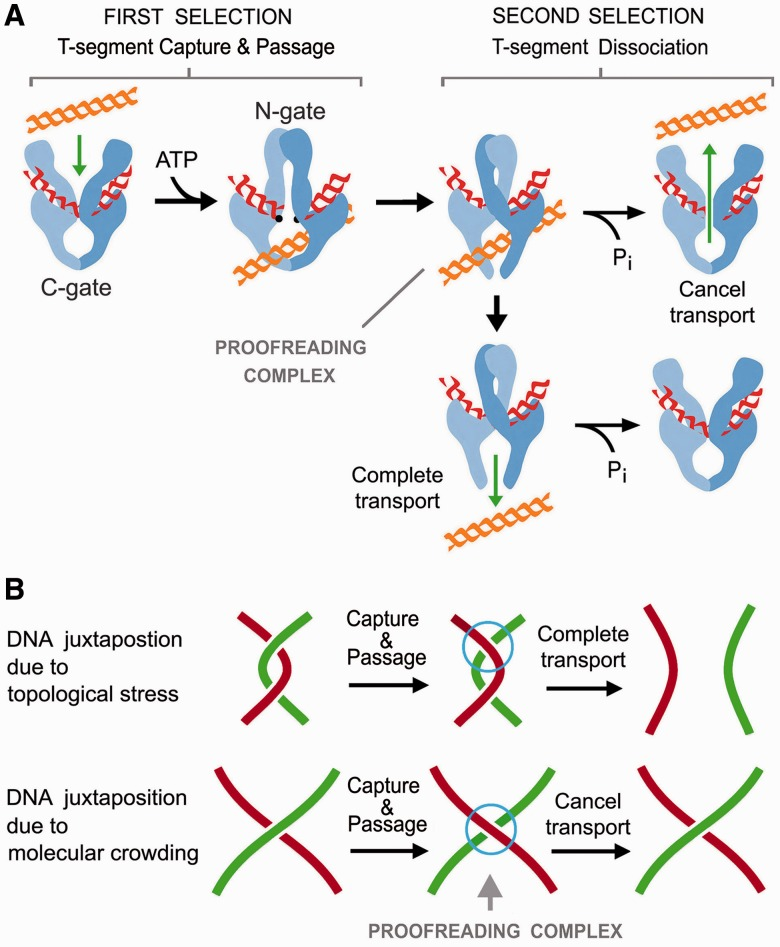
\includegraphics[width=.22\textwidth]{topoisomerase-II.jpeg}

\myem{사진출처: \cite{topo}}
\end{wrapfigure}
생명체의 DNA가 가지고 있는 이중나선구조는 DNA를 형태적으로 안정하게 유지시키는 반면, 이로 인해 꼬임이 발생한다.
이 꼬임은 복제와 전사가 일어 날 때 진행 과정을 방해하는 요소 중 하나이다.
\myem{DNA 회전효소(topoisomerase)}는 전사나 복제 과정 중,
복제 분기점 앞에서 DNA를 인산의 결합을 절단하고 회전시켜 과도한 꼬임을 완화시킨다.
이 과정에서 과도한 꼬임이 풀리며, 절단된 DNA도 재결합된다.\cite{campbell}

복제과정에서 꼬임의 풀림은 매듭이론에서 엇갈림 변환으로 설명할 수 있다.
따라서 매듭의 엇갈림에 대한 연구를 통해 DNA 복제과정을 이해할 수 있다.
본 연구에서는 여러 가지 매듭 중에서 특정 가상 토러스 매듭의 풀림수에 대하여 탐구하였다.
}


\block{정의 및 선행연구}
{
\mysection{가상 매듭 다이어그램(Virtual Knot Diagrams)}
\bigskip
\begin{center}
\begin{tabu} to .8\linewidth{X[1.3,m,c] X[.5,c] X[1.3,m,c] X[.5,c] X[2,m,c] X[.5,c] X[2,m,c] X[.5,c]}

\includegraphics[width=\linewidth]{crossing}
& & 
\includegraphics[width=\linewidth]{v_crossing}
& & 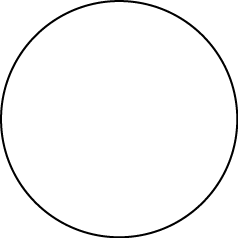
\includegraphics[width=\linewidth]{unknot}
& & 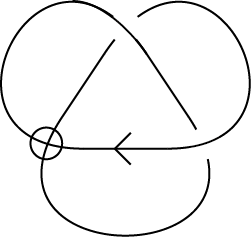
\includegraphics[width=\linewidth]{oriented_v_knot} 
&\\
\myem{엇갈림} & \multicolumn3{c}{\myem{가상 엇갈림}} & \myem{풀린매듭} & \multicolumn3{c}{\myem{방향 가상 고리 다이어그램}}\\
%\myem{(Crossing)} & \multicolumn3{c}{\myem{(Virtual Crossing)}} & \myem{(Unknot)} & \multicolumn3{c}{\myem{(Oriented Virtual Knot Diagram)}}
\end{tabu}
\end{center}

\bigskip\bigskip
\mysection{가상 매듭의 동치변환(Equivalence Moves of Virtual Knots)}
\bigskip
\begin{center}
\begin{tabu} to \linewidth{X[4.5,m,c] X[.1,m,c] X[2.5,m,c]}
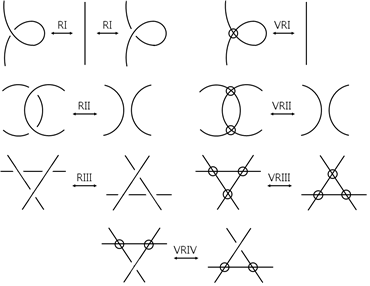
\includegraphics[width=\linewidth]{reide}
& & 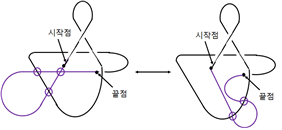
\includegraphics[width=\linewidth]{detour}
\\
\myem{확장 라이데마이스터 변환} & & \myem{우회 변환}\\
%\myem{(Generalized Reidemeister Moves)} & & \myem{(Detour Move)}
\end{tabu}
\end{center}


\bigskip\bigskip
\mysection{풀림수(Unknotting Number)}
\bigskip
\begin{center}
\begin{tabu} to .7\linewidth{X[2,m,c] X[1,m,c] X[2,m,c] X[2,m,c] X[2,m,c] X[1,m,c] X[2,m,c]}

\includegraphics[width=\linewidth]{crossing}
& $\Longrightarrow$ & 
\includegraphics[width=\linewidth]{crossing2} &
& 
\includegraphics[width=\linewidth]{crossing}
& $\Longrightarrow$ & 
\includegraphics[width=\linewidth]{v_crossing} \\
\multicolumn3{c}{\myem{엇갈림 변환}} &
& \multicolumn3{c}{\myem{가상화}} \\
%\multicolumn3{c}{\myem{(Crossing Change)}} & & \multicolumn3{c}{\myem{Virtualization}} \\
\end{tabu}
\end{center}

\myem{가상 풀림수(Virtual Unknotting Number)}, \myem{$\mathrm{vu}(K)$}:\\
\hspace*{2em}가상 매듭 $K$를 풀린 매듭으로 만드는데 필요한 최소한의 엇갈림 변환의 횟수

\myem{가상화 풀림수(Virtualization Unknotting Number)}, \myem{$\mathrm{vvu}(K)$}:\\
\hspace*{2em}가상 매듭 $K$를 풀린 매듭으로 만드는데 필요한 최소한의 가상화 횟수


\bigskip\bigskip
\mysection{가우스 다이어그램(Gauss Diagram)과 $P$-불변량(Invariant)}
\bigskip
\begin{center}
\begin{tabu} to .9\linewidth{X[2,m,c] X[.5,m,c] X[3,m,c] X[.5,m,c] X[4,m,c] }
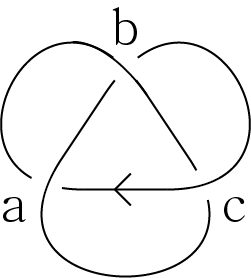
\includegraphics[width=\linewidth]{gauss1}
 &  & 
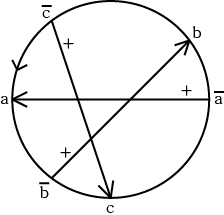
\includegraphics[width=\linewidth]{gauss2} & & 
$\displaystyle P(K) = \sum_{\substack{c\in A(G(K))\\ i(c)\neq 0}}\operatorname{sign}(c)t^{|i(c)|}$\\
\multicolumn3{c}{\myem{가우스 문자열}} & & \myem{$P$-불변량}\\
\multicolumn3{c}{\myem{$a+\overline{b}+c+\overline{a}+b+\overline{c}+$}} & & 
\end{tabu}
\end{center}
}



\column{0.5}

\block{}
{
\bigskip\bigskip
\mysection{토러스 매듭(Torus Knots)}
\bigskip
\begin{center}
\begin{tabu} to .9\linewidth{X[3,m,c] X[.2,m,c] X[3,m,c] X[.2,m,c] X[3,m,c]}
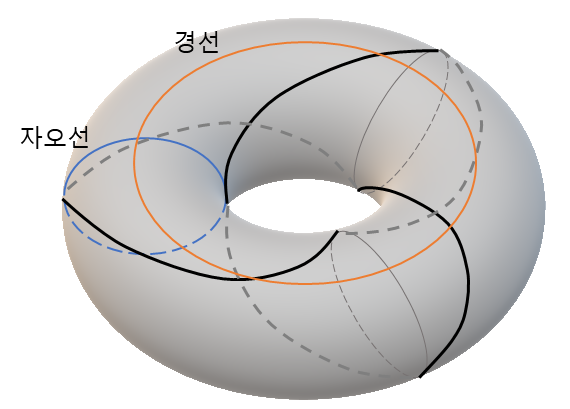
\includegraphics[width=\linewidth]{torus1}
 &  &

\includegraphics[width=\linewidth]{torus2}
 &  &

\includegraphics[width=\linewidth]{vt542}\\
\myem{토러스 매듭}
 &  &
\myem{$(7,5)$-토러스 매듭}
 &  &
\myem{가상 토러스 매듭 $VT_{5,4}^2$}
\end{tabu}
\end{center}


\bigskip\bigskip
{\textbf{\color{BrickRed}\sf정리\cite{v_bridge}.} 방향 가상 매듭 $𝐾$의 $P$-불변량이 $\displaystyle P(K)=\sum_{m\in\mathbf{N}}b_mt^m$일 때, 가상 풀림수의 하계는
\[
{\color{BrickRed}\mathrm{vu}(K)\ge \frac12\sum_{m\in\mathbf{N}}|b_m|}
\]
}
}



\block{연구내용 및 결과}
{
\mysection{$VT_{p,q}^{q-1}$의 풀림수}
\bigskip
{\textbf{\color{BrickRed}\sf정리.}
가상 토러스 매듭 $VT_{p,q}^{q-1}$의 가상 풀림수 $\mathrm{vu}\left(VT_{p,q}^{q-1}\right)$의 하계는
\[
{\color{BrickRed}\mathrm{vu}\left(VT_{p,q}^{q-1}\right)\le \frac{p-1}{2}-\frac{\gcd(p,q-1)-1}{2}}
\]
}
\vspace{-1em}
\begin{center}
\begin{tabu} to .9\linewidth{X[2,m,c] X[.1,m,c] X[2,m,c] X[.1,m,c] X[3,m,c]}
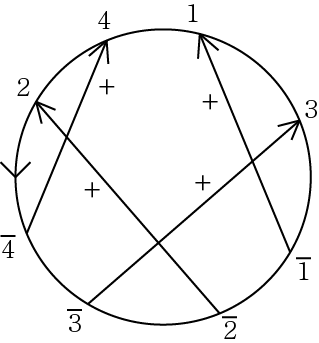
\includegraphics[width=.8\linewidth]{GVT532}
 &  &
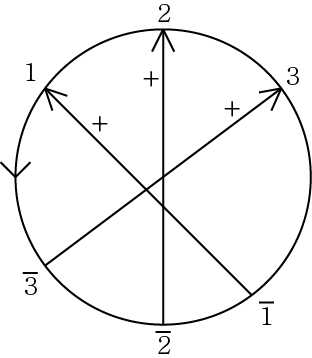
\includegraphics[width=.8\linewidth]{GVT432}
 &  &
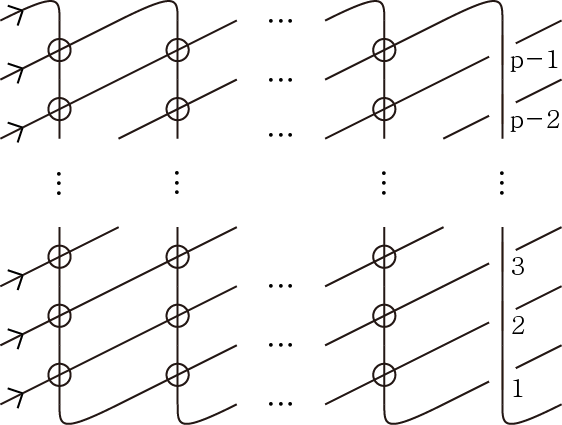
\includegraphics[width=.8\linewidth]{VTpqq-1}\\
\myem{$G\left(VT_{5,3}^2\right)$}
 &  &
\myem{$G\left(VT_{4,3}^2\right)$}
 &  &
\myem{$VT_{p,q}^{q-1}$}
\end{tabu}
\end{center}


\bigskip
\bigskip
{\textbf{\color{BrickRed}\sf정리.}
가상 토러스 매듭 $VT_{p,q}^{q-1}$의 가상 풀림수 $\mathrm{vu}\left(VT_{p,q}^{q-1}\right)$의 상계는
\[
{\color{BrickRed}\mathrm{vu}\left(VT_{p,q}^{q-1}\right)\ge \frac{p-1}{2}-\frac{\gcd(p,q-1)-1}{2}}
\]
}
\vspace{-1em}
\begin{center}
\begin{tabu} to .9\linewidth{X[3,m,c] X[.1,m,c] X[2,m,c]}
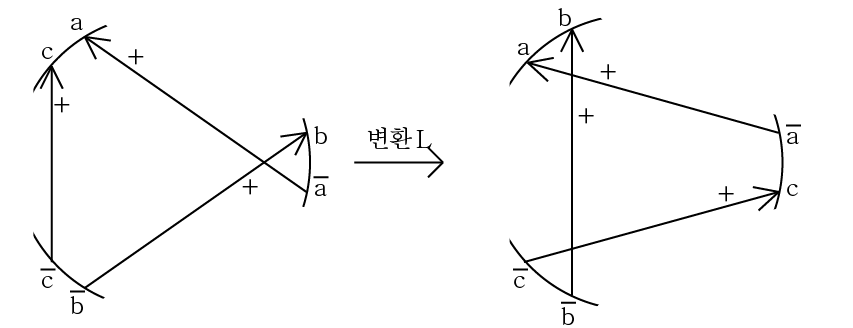
\includegraphics[width=.8\linewidth]{l_move_gauss}
 &  &
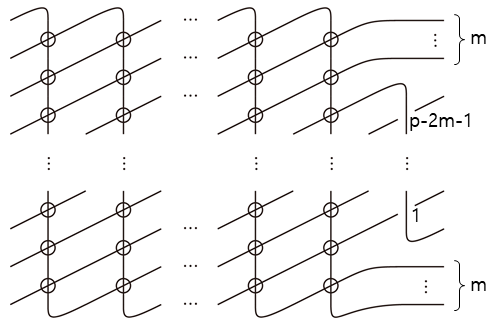
\includegraphics[width=.8\linewidth]{rvt}\\
\myem{변환 $L$}
 &  &
\myem{$RVT_{p,q}^m$}\\
\multicolumn3{c}{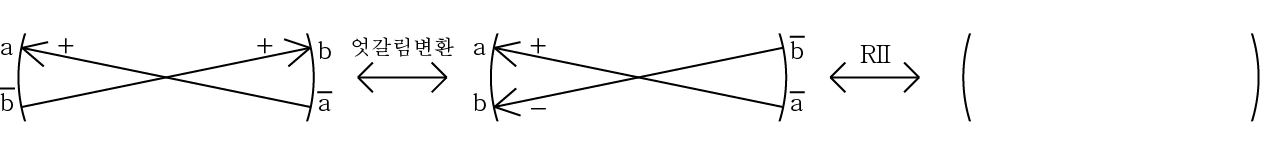
\includegraphics[width=.8\linewidth]{p_move}}\\
\multicolumn3{c}{\myem{변환 $P$}}
\end{tabu}
\end{center}


\mysection{$VT_{p,q}^{q-1}$의 가상화 풀림수}
\bigskip
{\textbf{\color{BrickRed}\sf정리.}
가상 토러스 매듭 $VT_{p,q}^{q-1}$에 대해 다음이 성립한다.
{\color{BrickRed}
\begin{quotation}
\textbf{1.} $\displaystyle \mathrm{vvu}\left(VT_{1,0}^{-1}\right)=0$
\qquad\qquad\quad\quad\quad
\textbf{2.} $\displaystyle \mathrm{vvu}\left(VT_{n,1}^{0}\right)=0$, $n\in\mathbf{N}$
\medskip

\textbf{3.} $\displaystyle \mathrm{vvu}\left(VT_{p,q}^{q-1}\right)\le(q-1)\left[\frac{p}{q}\right]+\mathrm{vvu}\left(VT_{p \mod q,\ q \mod (p \mod q)}^{(q \mod (p \mod q))-1}\right)$
\end{quotation}
}
}


\mysection{$VT_{p,q}^{q-2}$의 풀림수}
\bigskip
{\textbf{\color{BrickRed}\sf정리.}
가상 토러스 매듭 $VT_{p,q}^{q-2}$에서 $kq \equiv -1 \mod p$가 되는 최소의 양의 정수가 $k$이면
{\color{BrickRed}\small
\[
\mathrm{vu}\left(VT_{p,q}^{q-2}\right)\ge (p-1) - \left[\frac{\min\left\{k,\frac{p-1}{2}\right\}\times\gcd(q-2,p)}{p}\right] - \left[\frac{\min\left\{p-1-k,\frac{p-1}{2}\right\}\times\gcd(q-2,p)}{p}\right] 
\]
}
}
\begin{center}
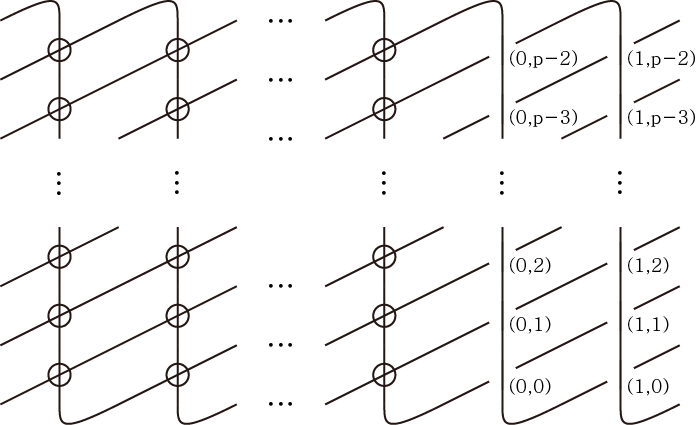
\includegraphics[width=.35\linewidth]{VTpqq-2}
\end{center}

}

\block{}
{\scriptsize
\nocite{*}
\bibliography{Virtual_Unkotting_Number_Torus}{}
\bibliographystyle{plain}

\begin{center}
\begin{tabu} to \linewidth{X[4.5,m,l] X[1,m,c] X[4.5,m,r]}

\includegraphics[width=.6\linewidth]{ksa}
 &  &

\includegraphics[width=.6\linewidth]{s_ict}
\end{tabu}
\end{center}
\vspace{-1em}
}



\end{columns}

\end{document}
\endinput
%%
%% End of file 

\block{}
{

}

\note[targetoffsetx=-8cm, targetoffsety=-9cm, width=25cm, innersep=1cm]
{
    \begin{wrapfigure}{r}{3cm}	
    \vspace{-23pt}
	\includegraphics[scale=3]{eu.jpg}
	
	\includegraphics[scale=3]{fp7.jpg}
	\end{wrapfigure}
	\textbf{Funding:} This research has received funding 
	from the People Programme (Marie Curie Actions) of the EU 7th Framework
	Programme (FP7/2007-2013), REA grant agreement no. 302868.
    
}
